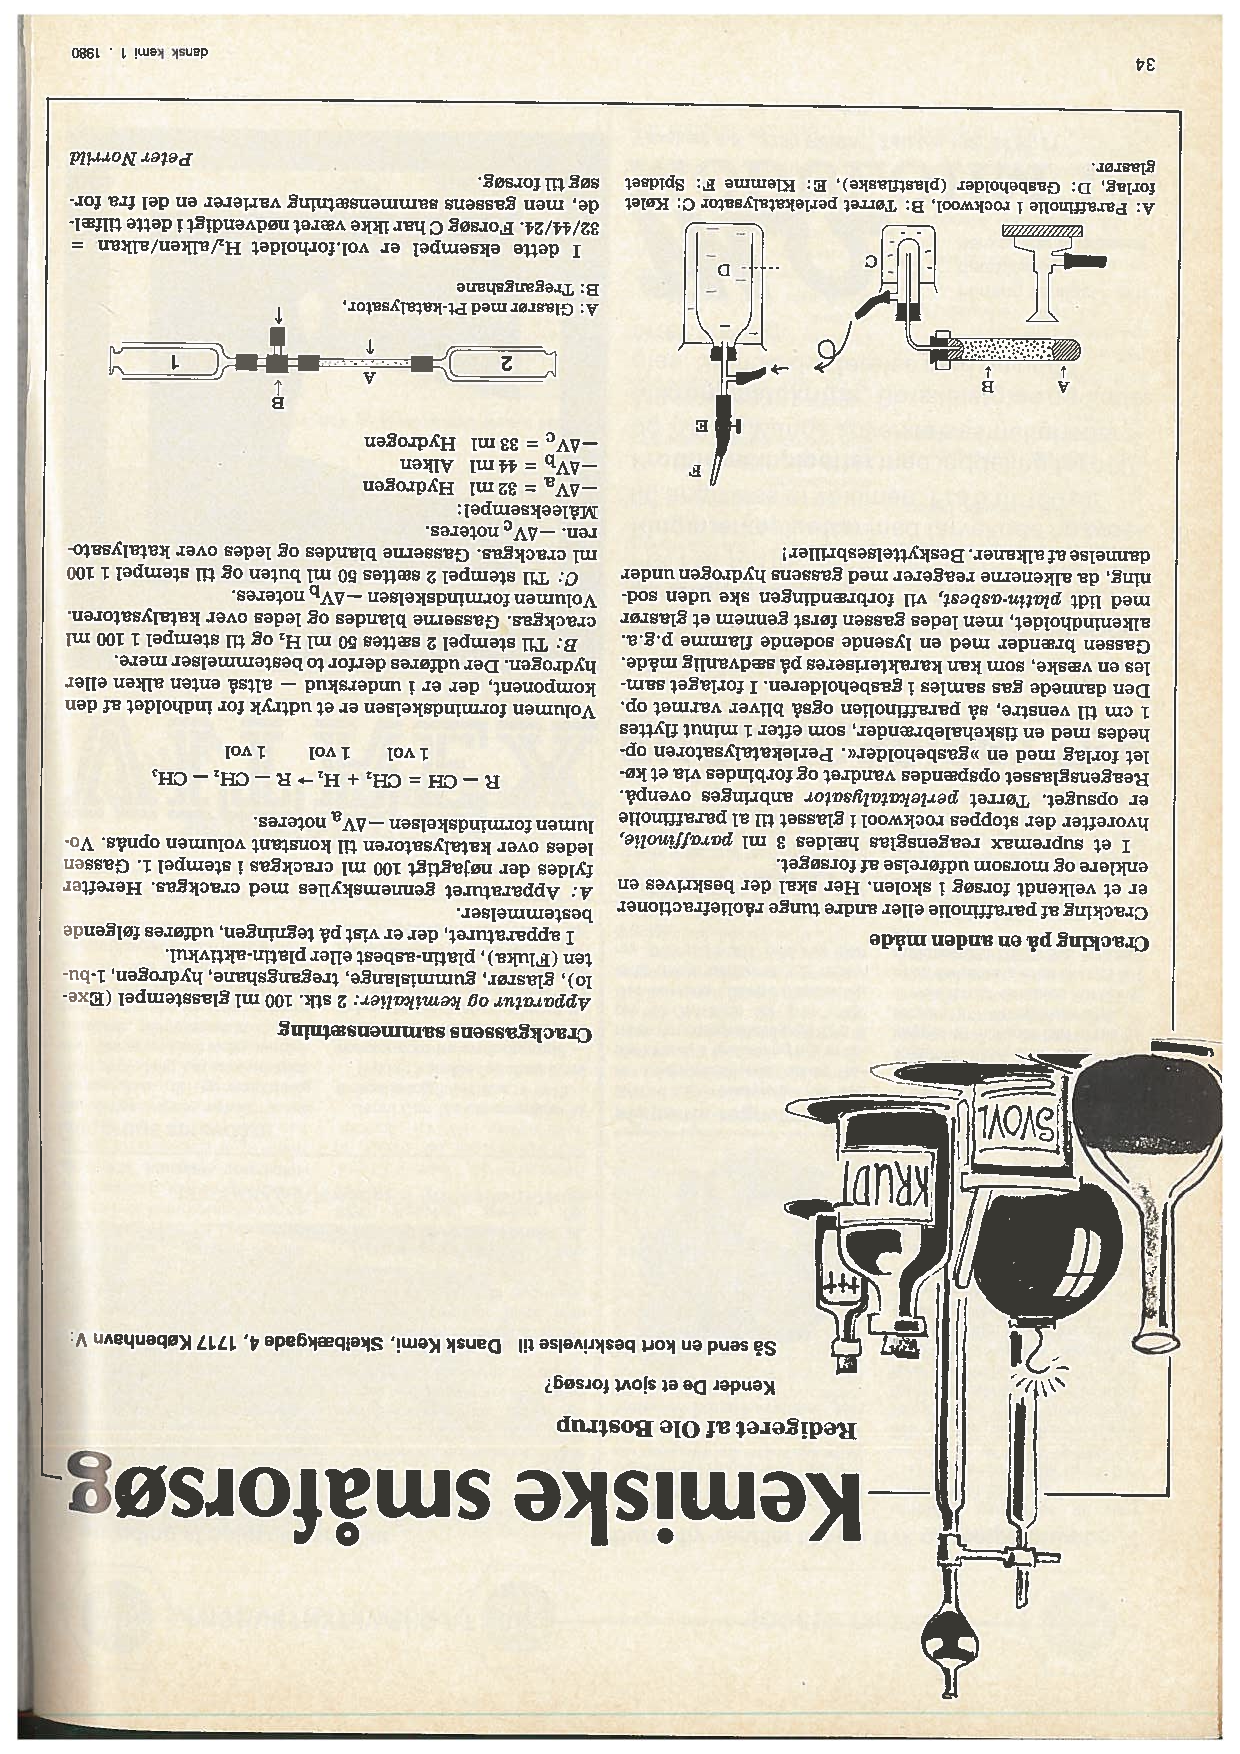
\includepdf[pages=-]{pdfs/1980-61-1-34.pdf}
\emne{Cracking på en anden måde}
\danskkemi{ dansk kemi vol 61 iss 1 p 34}
\forfatter{Peter Norrild}



Cracking af paraffinolie eller andre tunge råoliefractioner er et velkendt
forsøg i skolen. Her skal der beskrives en enklere og morsom udførelse af
forsøget.

I et supremax reagensglas hældes 3 ml paraffinolie, hvorefter der stoppes
rockwool i glasset til al paraffinolie er opsuget. Tørret perlekatalysator
anbringes ovenpå. reagensglasset opspændes vandret og forbindes via et kølet
forlag med en "gasbeholder". perlekatalysatoren ophedes med en fiskehalebrænder,
som efter 1 minut flyttes 1 cm til venstre, så paraffinolien også bliver varmet
op. Den dannede gas samles i gasbeholderen. I forlaget samles en væske, som kan
karakteriseres på sædvanlig måde. Gassen brænder med en lysende sodende flamme
p.g.a. alkenindholdet, men ledes gassen først gennem et glasrør med lidt
platin-asbest, vil forbrændingen ske uden sodning, da alkenerne reagerer med
gassens hydrogen under dannelse af alkaner. Beskyttelsesbriller!

\deloverskrift{Crackgassens sammensætning}

Apparatur og kemikalier: 2 stk. 100 ml glasstempel (Exelo), glasrør,
gummislange, tregangshane, hydrogen, 1-buten (Fluka), platin-asbest
eller platin-aktivkul.
I apparaturet, der er vist på tegningen, udføres følgende bestemmelser.
A: Apparaturet gennemskylles med crackgas. Herefter fyldes der nøjagtigt
100 ml crackgas i stempel 1. Gassen ledes over katalysatoren til konstant
volumen opnås. Volumen formindskelsen -Delta Va noteres.

R-CH=CH2 + H2 -> R-CH2-CH3
1 vol 1 vol 1 vol

Volumen formindskelsen er et udtryk for indholdet af den komponent, der
er i underskud - altså enten alekn eller hydrogen. Der udføres derfor to bestemmelser mere.
B: Til stempel 2 sættes 50 ml H2 og til stempel 1 100 ml crackgas.
Gassernes blandes og ledes over katalysatoren. Volumen formindskelsen
-Delta Vb noteres.
C: Til stempel 2 sættes 50 ml buten og til stempel 1 100 ml
crackgas. Gasserne blandes og ledes over katalysatoren. - Delta Vc
noteres.
Måleeksempel:
- Delta Va = 32 ml Hydrogen
-Delta Vb = 44 ml Alken
-Delta Vc = 33 ml Hydrogen

I dette eksempel er vol.forholdet H2/alken/alkan = 32/44/24.
Forsøg C har ikke været nødvendigt i dette tilfælde, men gassens
sammensætning varierer en del fra forsøg til forsøg.

noter til illustration 1:
A: Paraffinolie i rockwool, B: Tørret perlekatalysator D: Kølet forlag,
D: Gasbeholder (plastflaske), E: Klemme F: Spidset glasrør.

Noter til illustration 2:
A: Glasrør med Pt-katalysator,
B: tregangshane
